\chapter{Anexos}
\label{cha:anexos}

\section{Territorios de prácticas participativas}
\label{sec:territorios}

Actualmente estoy dividiendo la información en un gran conjunto de Diagramas de Venn (en realidad más bien Esferas de Venn):\footnote{Traducido con \url{www.deepl.com/translator} desde \url{www.github.com/ParticipatoryOrgs/Participatory-Organizations-Overview-and-Taxonomy}}

La esfera más grande es la de los Ecosistemas Participativos, que tienen una serie de prácticas para apoyar los sistemas regenerativos de un bien común, así como una política cultural para aumentar la participación a todos los niveles, y para incentivar contra la tragedia de los bienes comunes y la desigualdad en la equidad.

Dentro de esa esfera se encuentran dos esferas de Venn, las Corporaciones Participativas y las Organizaciones Participativas. Tienen mucho en común, pero las Corporaciones Participativas tienen más que ver con el mantenimiento y crecimiento del capital financiero, mientras que las Organizaciones Participativas están más enfocadas en el mantenimiento y crecimiento de las comunidades.

Dentro de la intersección de las esferas de las Corporaciones y Organizaciones Participativas hay un número de burbujas más pequeñas. Hay una gobernanza participativa, operaciones participativas y una visión y cultura participativas.

La gobernanza participativa aumenta el compromiso de las partes interesadas al hacerlas participar en la elaboración de políticas. Existe una gran variedad de estos procesos. Lo que se conoce como \emph{Toma de Decisiones por Consenso} es una esfera que está más cerca del lado de las Organizaciones Participativas, pero también cerca del lado de la Visión. Hubo bastante innovación en estos procesos en el movimiento \emph{New Paradyne Management} que terminó a mediados de los 90 debido al boom de las \emph{punto com} que no requirió una gran participación o incluso una gran gestión.

Operaciones Participativas se centra más en tener más ojos en las tácticas y la logística. Los procesos Lean y Agile encajan aquí, Intrapreneuring puede así como una serie de otros procesos de gestión de proyectos.

La Gobernabilidad Dinámica es una esfera de Venn que se encuentra mayormente dentro de la Gobernabilidad Participativa, pero más cerca del lado de las Operaciones Participativas que del lado de la visión. Dentro de eso está la Sociocracia que se inclina fuertemente hacia las Organizaciones Participativas en la preservación del capital comunitario y social y también cerca de la Visión y Cultura Participativa. La Holacracia es también una forma de Gobierno Dinámico, pero se inclina hacia el lado corporativo, pero también trata de funcionar mucho más en el espacio de Operaciones Participativas. La Holacracia apoya más la esfera de la Política que las Operaciones. La sociocracia también apoya más a la esfera de la política, pero en gran medida da flexibilidad a la esfera operativa.

Las prácticas participativas pueden dividirse en 3 grandes áreas: Sistemas participativos, participatory equity y gobernanza participativa.

Algunos principios:\todo{¿y por qué en inglés?}

\begin{itemize}
\item \emph{Act}: You Already Have Permission
\item \emph{Flow}: Every Idea Is Playdough
\item \emph{Open}: Everything Is Transparent
\item \emph{Accept}: It Isn't Easy Being Green
\item \emph{Share}: Communication Is Oxygen
\end{itemize}

\begin{figure}[htbp]
	\centering
	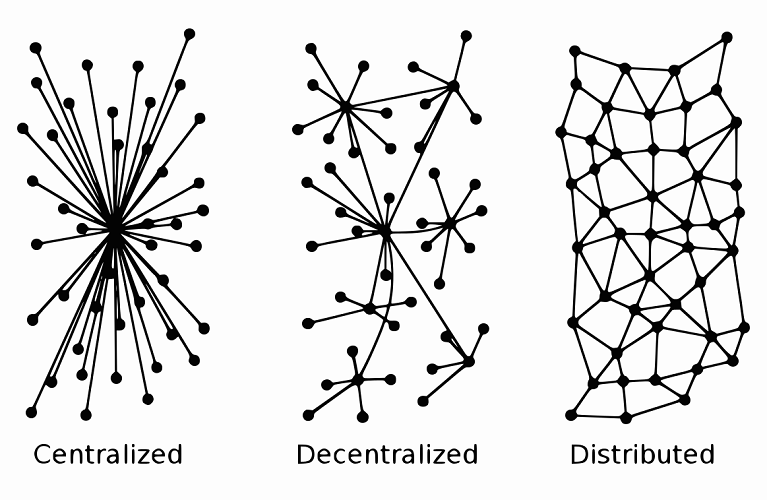
\includegraphics[width=.9\linewidth]{decentralized.png}
	\caption{Centralizado, descentralizado, distribuido.}
	\label{fig:descentralizado}
\end{figure}

\section{Tiranía de la falta de estructuras}
\label{sec:tirania}

Es importante enfatizar el patrón negativo discutido en el famoso ensayo de Jo Freeman de 1970 \emph{The Tyranny of Structureless}. Usando las lecciones del movimiento feminista de los años 60, evitar la estructura puede en realidad reforzar las estructuras, y a menudo de manera no beneficiosa, enmascarando los abusos de poder:

\begin{quotation}
	Contrariamente a lo que nos gustaría creer, no existe tal cosa como un grupo sin estructura. Cualquier grupo de personas de cualquier naturaleza que se reúna por cualquier período de tiempo y con cualquier propósito se estructurará inevitablemente de alguna manera. La estructura puede ser flexible; puede variar con el tiempo; puede distribuir las tareas, el poder y los recursos entre los miembros del grupo de manera uniforme o desigual. Pero se formará independientemente de las habilidades, personalidades o intenciones de las personas involucradas. El hecho mismo de que somos individuos, con diferentes talentos, predisposiciones y antecedentes, hace que esto sea inevitable. Sólo si nos negamos a relacionarnos o a interactuar sobre cualquier base, podremos aproximarnos a la falta de estructura - y esa no es la naturaleza de un grupo humano.

	Esto significa que luchar por un grupo sin estructura es tan útil y engañoso como apuntar a una noticia \emph{objetiva}, a una ciencia social \emph{sin valor} o a una economía \emph{libre}. Un grupo de laissez faire es tan realista como una sociedad de \emph{laissez faire}; la idea se convierte en una cortina de humo para que los fuertes o los afortunados establezcan una hegemonía incuestionable sobre otros. Esta hegemonía puede establecerse tan fácilmente porque la idea de falta de estructura no impide la formación de estructuras informales, sólo formales. De manera similar, la filosofía del \emph{laissez faire} no impidió que los económicamente poderosos establecieran el control sobre los salarios, los precios y la distribución de los bienes; sólo impidió que el gobierno lo hiciera. Por lo tanto, la falta de estructura se convierte en una forma de enmascarar el poder, y dentro del movimiento de las mujeres es por lo general más fuertemente defendido por aquellos que son los más poderosos (sean o no conscientes de su poder). Mientras la estructura del grupo sea informal, las reglas de cómo se toman las decisiones son conocidas sólo por unos pocos y la conciencia del poder se limita a aquellos que conocen las reglas. Aquellos que no conocen las reglas y no son elegidos para la iniciación deben permanecer confundidos, o sufrir de delirios paranoicos de que algo está sucediendo de lo que no son del todo conscientes.
\end{quotation}

También:

\begin{itemize}
\item \url{http://www.wired.com/2014/03/tyranny-flatness/}
\item \url{https://en.wikipedia.org/wiki/Flat\_organization\#Criticisms}
\item \url{https://theanarchistlibrary.org/library/cathy-levine-the-tyranny-of-tyranny}
\end{itemize}

\section{Bienes comunes}
\label{sec:org695eb10}

Las organizaciones participativas suelen tener que gestionar recursos en común al interior de la organización en su conjunto (activos, presupuestos, tiempo, etc.), o están participando en bienes públicos compartidos pero limitados que, junto con otras organizaciones, pueden ser tangibles (aire, recursos, etc.) o intangibles (conocimiento, código abierto, etc.).

En 2009, Elinor Ostrom recibió el Premio Nobel de Economía por su análisis de la gobernanza económica, especialmente de los bienes comunes. En ese sentido, enumeró ocho principios para una gestión eficaz contra la tragedia de los bienes comunes. Estos son muy útiles para las organizaciones participativas:

\begin{enumerate}
	\item[1A.] Definir el uso autorizado

	\item[1B.] Definir los límites de los bienes comunes

	\item[2A.] Hacer que los costes sean proporcionales

	\item[2B.] Pagar todos los gastos

	\item[3A.] Decidir inclusivamente

	\item[3B.] Adaptarse localmente

	\item[4A.] Compartir conocimientos

	\item[4B.] Monitoreo efectivo

	\item[5 .] Responsabilizar (\emph{hold accountable})

	\item[6 .] Resolver rápidamente los conflictos

	\item[7 .] Gobernar localmente

	\item[8 .] Conectar y coordinar con sistemas relacionados
\end{enumerate}

\section{Referencias del apartado}
\label{sec:ref07}

\begin{itemize}
	\item How Commons Can Flourish: \url{https://commons.blog/2012/08/18/how-commons-can-flourish/}
	\item The Antifragile: Things That Gain from Disorder: \url{https://cpor.org/af/Taleb\_Antifragile.pdf}
	\item Herramientas del partido pirata argentino: \url{https://utopia.partidopirata.com.ar/democracia\_directa.html}
	\item Algoritmos para predecir cooperación social: \url{http://news.harvard.edu/gazette/story/2017/03/harvard-scientists-help-develop-algorithm-that-predicts-social-cooperation/}
	\item Movimiento OPEN: \url{http://open.co/}
	\item Agentes de innovación en México - CIDE: \url{https://es.slideshare.net/mobile/DapCide/advancing-innovation-mexicos-innovation-agents-eng} 
	\item Ciencia de redes, por Laszlo Barabási: \url{http://barabasi.com/networksciencebook/}
	\item Marcos para diseño organizacional: \url{http://isites.harvard.edu/fs/docs/icb.topic608877.files/Class\%20Nine\%20Reading/CLC\_Frameworks\_for\_Organizational\_Design.pdf}
	\item De capos y rodeos, ¿por qué nada funciona?: \url{https://www.northatlanticbooks.com/blog/of-warlords-and-rodeos-why-nothing-works/}
	\item Problem Driven Iterative Adaptation (vs other mainstream approaches for public policy): \url{https://www.hks.harvard.edu/index.php/centers/cid/programs/building\_state\_capability/what-is-pdia}
	\item \url{https://framasoft.org}
	\item \url{http://unenumerated.blogspot.com/2017/02/money-blockchains-and-social-scalability.html}
	\item \url{http://unenumerated.blogspot.com/2006/11/wet-code-and-dry.html}
\end{itemize}